\newcommand{\uco}{\fun{uco}}
\newcommand{\lfp}{\fun{lfp}}
\newcommand{\wide}{\nabla}

\chapter{Teoria dei reticoli}\label{chap:teoriareticoli}

\section{Poset}

\begin{definition}[Poset]
Un \emph{insieme parzialmente ordinato} o \emph{poset} è una struttura $\struct{P, \sqsubseteq}$ tale che $P$ è un insieme e $\sqsubseteq$ è una relazione binaria su $P$ che gode di proprietà \emph{riflessiva}, \emph{antisimmetrica} e \emph{transitiva}. 
\end{definition}

In una relazione d'ordine parziale $\sqsubseteq$ non è detto che tra due elementi $x,y \in P$ questi siano confrontabili, cioè che valga $x \sqsubseteq y \lor y \sqsubseteq x$. In questo caso si scrive $x || y$. Se tutti gli elementi dell'insieme sono a due a due confrontabili, la relazione d'ordine si dice \emph{totale} e viene indicata col simbolo $\le$. 

Esempi di poset le strutture $\struct{\mathbb{Z}, \le}$ (che è anche un insieme totalmente ordinato), la struttura $\struct{\wp(S), \subseteq}$ formata dall'insieme delle parti di un insieme $S$ e la relazione di inclusione insiemistica (Figura~\ref{fig:poset-parti}), ma anche la struttura $\struct{\{1,2,3,4,6,12\}, \mathbf{divide}}$.

\begin{figure}[htbp]
    \centering
    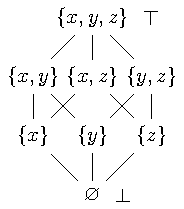
\includegraphics{appendici/immagini/poset-parti.pdf}
    \caption{Poset $\struct{\wp(S), \subseteq}$ con $S = \{x,y,z\}$}
    \label{fig:poset-parti}
\end{figure}

\begin{definition}[Elementi top e bottom]
All'interno di un poset $\struct{P, \sqsubseteq}$ si può individuare, se esiste, l'elemento top $\top \in P$ tale che $\forall x \in P . x \le \top$. Se l'elemento $\top$ esiste, è unico. L'elemento bottom $\bot$ è definito in modo duale.
\end{definition}

All'interno del poset $\struct{\wp(S), \subseteq}$ l'elemento top è $\top = S$ e il bottom è $\bot = \varnothing$. All'interno del poset $\struct{\mathbb{Z}, \le}$ non esiste l'elemento top ma esiste l'elemento bottom $\bot = 0$. Se ad $\mathbb{Z}$ aggiungiamo un ulteriore elemento $\infty$ tale che $\forall n \in \mathbb{Z} . n < \infty$ allora questo elemento funge da top per la nuova struttura $\struct{\mathbb{Z} \cup \{ \infty \}, \le}$ creata.

\begin{definition}[Least upper bound]
L'operazione di \emph{least upper bound} (o \emph{lub}, \emph{join}, \emph{estremo superiore}) tra due elementi $x,y \in P$ di un poset $\struct{P, \sqsubseteq}$ se esiste è l'elemento $\join[x][y] = z \in P$ tale che:
\begin{itemize}
    \item $\join[x][y]$ è maggiorante di $x$ e $y$ ($x,y \sqsubseteq \join[x][y]$);
    \item $\join[x][y]$ è il più piccolo maggiorante di $x$ e $y$ ($\forall m \in P . (x,y \sqsubseteq m \to \join[x][y] \sqsubseteq m)$);
    \item $\join[x][y]$ è unico.
\end{itemize}
\end{definition}

\begin{definition}[Greatest lower bound]
L'operazione di \emph{greatest lower bound} (o \emph{glb}, \emph{meet}, \emph{estremo inferiore}) è definito in modo duale al lub e di indica con $\meet[x][y]$ per $x,y \in P$.
\end{definition}

Il join (e il meet) di due elementi del poset può non essere definito per due motivi: \emph{l'elemento manca} (in $\struct{\{1,2,3,4,6,12,13\}, \mathbf{divide}}$ l'elemento $\join[12][13]$ non è definito poichè non c'è elemento maggiorante di entrambi) oppure \emph{non è rispettata la condizione di unicità} (se ci sono più maggioranti non confrontabili tra loro).

\begin{definition}[Catena]
Un sottoinsieme $C \subseteq P$ del poset $\struct{P, \sqsubseteq}$ è detto \emph{catena} se gli elementi di $C$ sono a due a due confrontabili tra loro. Il duale della catena è l'anticatena (elementi non confrontabili tra loro).  
\end{definition}

\begin{definition}[Condizione ACC]
Una catena $C$ soddisfa la \emph{ascending chain condition} se $C$ è un insieme finito oppure se da un certo $n$ in poi si ha $\forall m > n . c_n = c_m$.
\end{definition}

\begin{definition}[Poset completo]
Un poset $\struct{P, \sqsubseteq}$ si dice completo (abbreviato \emph{c.p.o.}) se per ogni sua catena $C$ anche infinita esiste l'estremo superiore $\join[C] \in P$.
\end{definition}

\subsection{Reticoli}

\begin{definition}[Reticolo]
Un reticolo è una struttura $\struct{P, \sqsubseteq, \join, \meet}$ nella quale $\struct{P, \sqsubseteq}$ è un poset, l'operazione binaria $\join$ effettua il lub, l'operazione $\meet$ effettua il glb ed 
\[ \forall x,y \in P \text{ sono definiti } \join[x][y], \meet[x][y] \in P \]
\end{definition}

\begin{definition}[Sottoreticolo]
Un sottoinsieme $Q \subseteq P$ del reticolo $\struct{P, \sqsubseteq, \join, \meet}$ è detto \emph{sottoreticolo} se $Q$ è chiuso per lub e glb ($\forall x,y \in Q . \join[x][y], \meet[x][y] \in Q$). 
\end{definition}

\begin{definition}[Reticolo completo]
Un reticolo che è anche c.p.o. viene detto reticolo completo.
\end{definition}

\subsection{Ordinamento pointwise di funzioni}

Date due funzioni $f_1, f_2 : C \to C$, il loro ordinamento parziale $\le$ è detto \emph{pointwise} se
\[ f_1 \le f_2 \iff \forall x \in C . f_1(x) \le f_2(x) \]

\subsection{Connessione di Galois}\label{sec:galois}

La definizione di connessione di Galois è presente alla Sezione~\ref{sec:galois-c}.

\begin{theorem}[Connessione di Galois come adjunctor]
La struttura è detta anche \emph{adjunctor} ($\alpha$ left adjoint, $\gamma$ right adjoint) poichè vale che
$$\forall c \in C, a \in A \; : \; \alpha(c) \preceq a \Leftrightarrow c \le \gamma(a)$$
\end{theorem}

\begin{theorem}[Connessione di Galois come funzioni additive e co-additive]
In una connessione di Galois la funzione $\alpha$ è additiva, cioè preserva l'operazione di join: 
$$\alpha\left(\join[X]\right) = \join[\alpha(X)] \text{ per ogni } X \subseteq C$$
e la funzione $\gamma$ è co-additiva, cioè preserva l'operazione di meet.
\end{theorem}

\begin{definition}[Inserzione di Galois]
Una connessione di Galois si dice \emph{inserzione di Galois} e si scrive $C \galoiS{\alpha}{\gamma} A$ se $\alpha \circ \gamma = \fun{id}$. Sono equivalenti le seguenti espressioni:
\begin{itemize}
    \item $C \galoiS{\alpha}{\gamma} A$;
    \item $\alpha$ è suriettiva;
    \item $\gamma$ è iniettiva.
\end{itemize}
\end{definition}

Le inserzioni di Galois sono molto simili alle connessioni. La differenza tra i due è che nelle connessioni è possibile che più elementi del dominio astratto corrispondano allo stesso elemento del dominio concreto. Togliendo questi elementi ``superflui" si ottiene una inserzione. Questo procedimento, detto \emph{reduction} è sempre possibile e consiste nell'identificare in una classe di equivalenza gli elementi del dominio astratto con la stessa concretizzazione.

\section{Closure operators}

Un'interpretazione astratta può essere definita equivalentemente come una inserzione di Galois oppure come un'operatore di chiusura. La teoria di questa sezione è presa da \cite{ranzato}, che espone questi concetti in modo più approfondito. 

\begin{definition}[Upper closure operator]
Una funzione $\rho: L \to L$ è detta \emph{upper closure operator} se
\begin{enumerate}
    \item monotona: $x \le y \to \rho(x) \le \rho(y)$;
    \item estensiva: $x \le \rho(x)$;
    \item idempotente: $\rho(\rho(x)) = \rho(x)$.
\end{enumerate}
\end{definition}

Dato un reticolo completo $C$, un'operatore di chiusura $\rho$ è determinato univocamente dalla sua immagine $\rho(C) = \mathrm{codomain}(\rho)$. L'immagine di un $\rho$ coincide con l'insieme dei suoi \emph{fixpoint}:
\[ \rho(y) = \meet[\{x \mid x \in \mathrm{codomain}(\rho) \land y \le x \}] \]

\begin{definition}[Famiglia di Moore]
Un sottoinsieme $X \subseteq L$ di un reticolo completo $L$ è detto \emph{famiglia di Moore} se $X$ è chiuso rispetto all'operazione di \emph{meet}, cioè
$$X = \mathcal{M}(X); \qquad \mathcal{M}(X) = \Big\{ \meet[S] \; \big| \; S \subseteq X \Big\}$$
\end{definition}

Viceversa, un'operatore $\rho$ sul dominio $J$ è un $\uco$ se e solo se il suo codominio $\rho(J) = K$ è una famiglia di Moore ed in quel caso $\rho(y) = \meet[\{x \mid x \in K \land y \le x \}]$. 

\subsection{Reticolo delle interpretazioni astratte}

Se $C$ è un reticolo completo, allora $\uco(C)$ forma un reticolo completo rispetto all'ordinamento pointwise con elemento $\top = \lambda x . \top$ e $\bot = \lambda x . x$. 

Dato $\rho \in \uco(C)$ ed un dominio astratto $A$, se $\rho(C)$ è isomorfico ad $A$ abbiamo $\iota: \rho(C) \to A$ ed $\iota^{-1} : A \to \rho(C)$. Allora la struttura
\[ \struct{\iota \circ \rho, C, A, \iota^{-1}} \]
è un'inserzione di Galois. Allo stesso tempo se $\struct{\gamma, C, A, \alpha}$ è un'inserzione di Galois allora $\rho_{A} = \gamma \circ \alpha$ è un $\uco(C)$.  

Definiamo l'insieme $\mathrm{Abs}(C)$ come l'insieme dei domini astratti di $C$. L'insieme forma un reticolo completo rispetto all'operazione di ordinamento
\[ A_1 \sqsubseteq A_2 
\iff \rho_{A_1} \subseteq \rho_{A_2} 
\iff \left( 
    \forall x . \rho_{A_1}(x) \le \rho_{A_2}(x)
\right) \]
e nel caso si dice che $A_1$ è più preciso (o più concreto) di $A_2$. La struttura $\struct{\mathrm{Abs}(C), \sqsubseteq}$ forma un reticolo completo detto \emph{reticolo delle interpretazioni astratte} ed è isomorfico al reticolo $\struct{\uco(C), \sqsubseteq}$. 

\section{Fixpoint}\label{sec:fixpoint}

\begin{definition}[Fixpoint]
Data $f:X \to X$, il punto $x \in X$ si definisce fixpoint se $f(x) = x$.
\end{definition}

\begin{definition}[Least fixed point]
Data $f:X \to X$, il punto $\lfp(f) = x \in X$ si definisce \emph{least fixed point} se per ogni $y$ fixpoint si ha $x \le y \to x = y$.
\end{definition}

\begin{theorem}[Teorema di Knaster-Tarski]
Data una funzione $f:L \to L$ monotona su un reticolo completo $\struct{L, \le}$ esiste un unico $\lfp(f)$.
\end{theorem}

E' possibile calcolare $\lfp(f)$ tramite il metodo iterativo:
$$\bot \le f(\bot) \le f^2(\bot) \le ... \le f^n(\bot) = \lfp(f) = f^{n+1}(\bot) = f^{n+2}(\bot) = ...$$

\section{Widening}

I domini concreti $C$ possono avere infiniti valori. I domini astratti che abbiamo visto possono avere valori finiti (dominio dei segni) o infiniti (dominio degli intervalli). A volte non è possibile garantire la convergenza dei calcoli su domini infiniti (non rispettando la condizione di ACC). Si definisce allora una funzione detta widening che garantisce la terminazione a costo di perdere ulteriore precisione.

\begin{definition}[Widening binario]
L'operatore di widening $\wide: P \times P \to P$ su un poset $\struct{P, \le}$ soddisfa le seguenti condizioni:
\begin{itemize}
    \item $\forall x,y \in P \, . \, x \le (\wide[x][y]) \land y \le (\wide[x][y])$;
    \item Per ogni catena $x_0 \le x_1 \le ...$ si definisce la catena \emph{non strettamente crescente} $y_0 = x_0, ..., y^{n+1} = \wide[x][y^n]$.
\end{itemize}
\end{definition}

L'operatore di widening non è commutativo ne associativo. L'iterazione col widening si svolge come segue:
$$x^0 = \bot \qquad x^{n+1} = \begin{cases} 
    x^n,                & f(x^n) \le x^n \\ 
    \wide[x^n][f(x^n)], & f(x^n) \not\le x^n \\
\end{cases}$$
